\documentclass[1p]{elsarticle_modified}
%\bibliographystyle{elsarticle-num}

%\usepackage[colorlinks]{hyperref}
%\usepackage{abbrmath_seonhwa} %\Abb, \Ascr, \Acal ,\Abf, \Afrak
\usepackage{amsfonts}
\usepackage{amssymb}
\usepackage{amsmath}
\usepackage{amsthm}
\usepackage{scalefnt}
\usepackage{amsbsy}
\usepackage{kotex}
\usepackage{caption}
\usepackage{subfig}
\usepackage{color}
\usepackage{graphicx}
\usepackage{xcolor} %% white, black, red, green, blue, cyan, magenta, yellow
\usepackage{float}
\usepackage{setspace}
\usepackage{hyperref}

\usepackage{tikz}
\usetikzlibrary{arrows}

\usepackage{multirow}
\usepackage{array} % fixed length table
\usepackage{hhline}

%%%%%%%%%%%%%%%%%%%%%
\makeatletter
\renewcommand*\env@matrix[1][\arraystretch]{%
	\edef\arraystretch{#1}%
	\hskip -\arraycolsep
	\let\@ifnextchar\new@ifnextchar
	\array{*\c@MaxMatrixCols c}}
\makeatother %https://tex.stackexchange.com/questions/14071/how-can-i-increase-the-line-spacing-in-a-matrix
%%%%%%%%%%%%%%%

\usepackage[normalem]{ulem}

\newcommand{\msout}[1]{\ifmmode\text{\sout{\ensuremath{#1}}}\else\sout{#1}\fi}
%SOURCE: \msout is \stkout macro in https://tex.stackexchange.com/questions/20609/strikeout-in-math-mode

\newcommand{\cancel}[1]{
	\ifmmode
	{\color{red}\msout{#1}}
	\else
	{\color{red}\sout{#1}}
	\fi
}

\newcommand{\add}[1]{
	{\color{blue}\uwave{#1}}
}

\newcommand{\replace}[2]{
	\ifmmode
	{\color{red}\msout{#1}}{\color{blue}\uwave{#2}}
	\else
	{\color{red}\sout{#1}}{\color{blue}\uwave{#2}}
	\fi
}

\newcommand{\Sol}{\mathcal{S}} %segment
\newcommand{\D}{D} %diagram
\newcommand{\A}{\mathcal{A}} %arc


%%%%%%%%%%%%%%%%%%%%%%%%%%%%%5 test

\def\sl{\operatorname{\textup{SL}}(2,\Cbb)}
\def\psl{\operatorname{\textup{PSL}}(2,\Cbb)}
\def\quan{\mkern 1mu \triangleright \mkern 1mu}

\theoremstyle{definition}
\newtheorem{thm}{Theorem}[section]
\newtheorem{prop}[thm]{Proposition}
\newtheorem{lem}[thm]{Lemma}
\newtheorem{ques}[thm]{Question}
\newtheorem{cor}[thm]{Corollary}
\newtheorem{defn}[thm]{Definition}
\newtheorem{exam}[thm]{Example}
\newtheorem{rmk}[thm]{Remark}
\newtheorem{alg}[thm]{Algorithm}

\newcommand{\I}{\sqrt{-1}}
\begin{document}

%\begin{frontmatter}
%
%\title{Boundary parabolic representations of knots up to 8 crossings}
%
%%% Group authors per affiliation:
%\author{Yunhi Cho} 
%\address{Department of Mathematics, University of Seoul, Seoul, Korea}
%\ead{yhcho@uos.ac.kr}
%
%
%\author{Seonhwa Kim} %\fnref{s_kim}}
%\address{Center for Geometry and Physics, Institute for Basic Science, Pohang, 37673, Korea}
%\ead{ryeona17@ibs.re.kr}
%
%\author{Hyuk Kim}
%\address{Department of Mathematical Sciences, Seoul National University, Seoul 08826, Korea}
%\ead{hyukkim@snu.ac.kr}
%
%\author{Seokbeom Yoon}
%\address{Department of Mathematical Sciences, Seoul National University, Seoul, 08826,  Korea}
%\ead{sbyoon15@snu.ac.kr}
%
%\begin{abstract}
%We find all boundary parabolic representation of knots up to 8 crossings.
%
%\end{abstract}
%\begin{keyword}
%    \MSC[2010] 57M25 
%\end{keyword}
%
%\end{frontmatter}

%\linenumbers
%\tableofcontents
%
\newcommand\colored[1]{\textcolor{white}{\rule[-0.35ex]{0.8em}{1.4ex}}\kern-0.8em\color{red} #1}%
%\newcommand\colored[1]{\textcolor{white}{ #1}\kern-2.17ex	\textcolor{white}{ #1}\kern-1.81ex	\textcolor{white}{ #1}\kern-2.15ex\color{red}#1	}

{\Large $\underline{11a_{205}~(K11a_{205})}$}

\setlength{\tabcolsep}{10pt}
\renewcommand{\arraystretch}{1.6}
\vspace{1cm}\begin{tabular}{m{100pt}>{\centering\arraybackslash}m{274pt}}
\multirow{5}{120pt}{
	\centering
	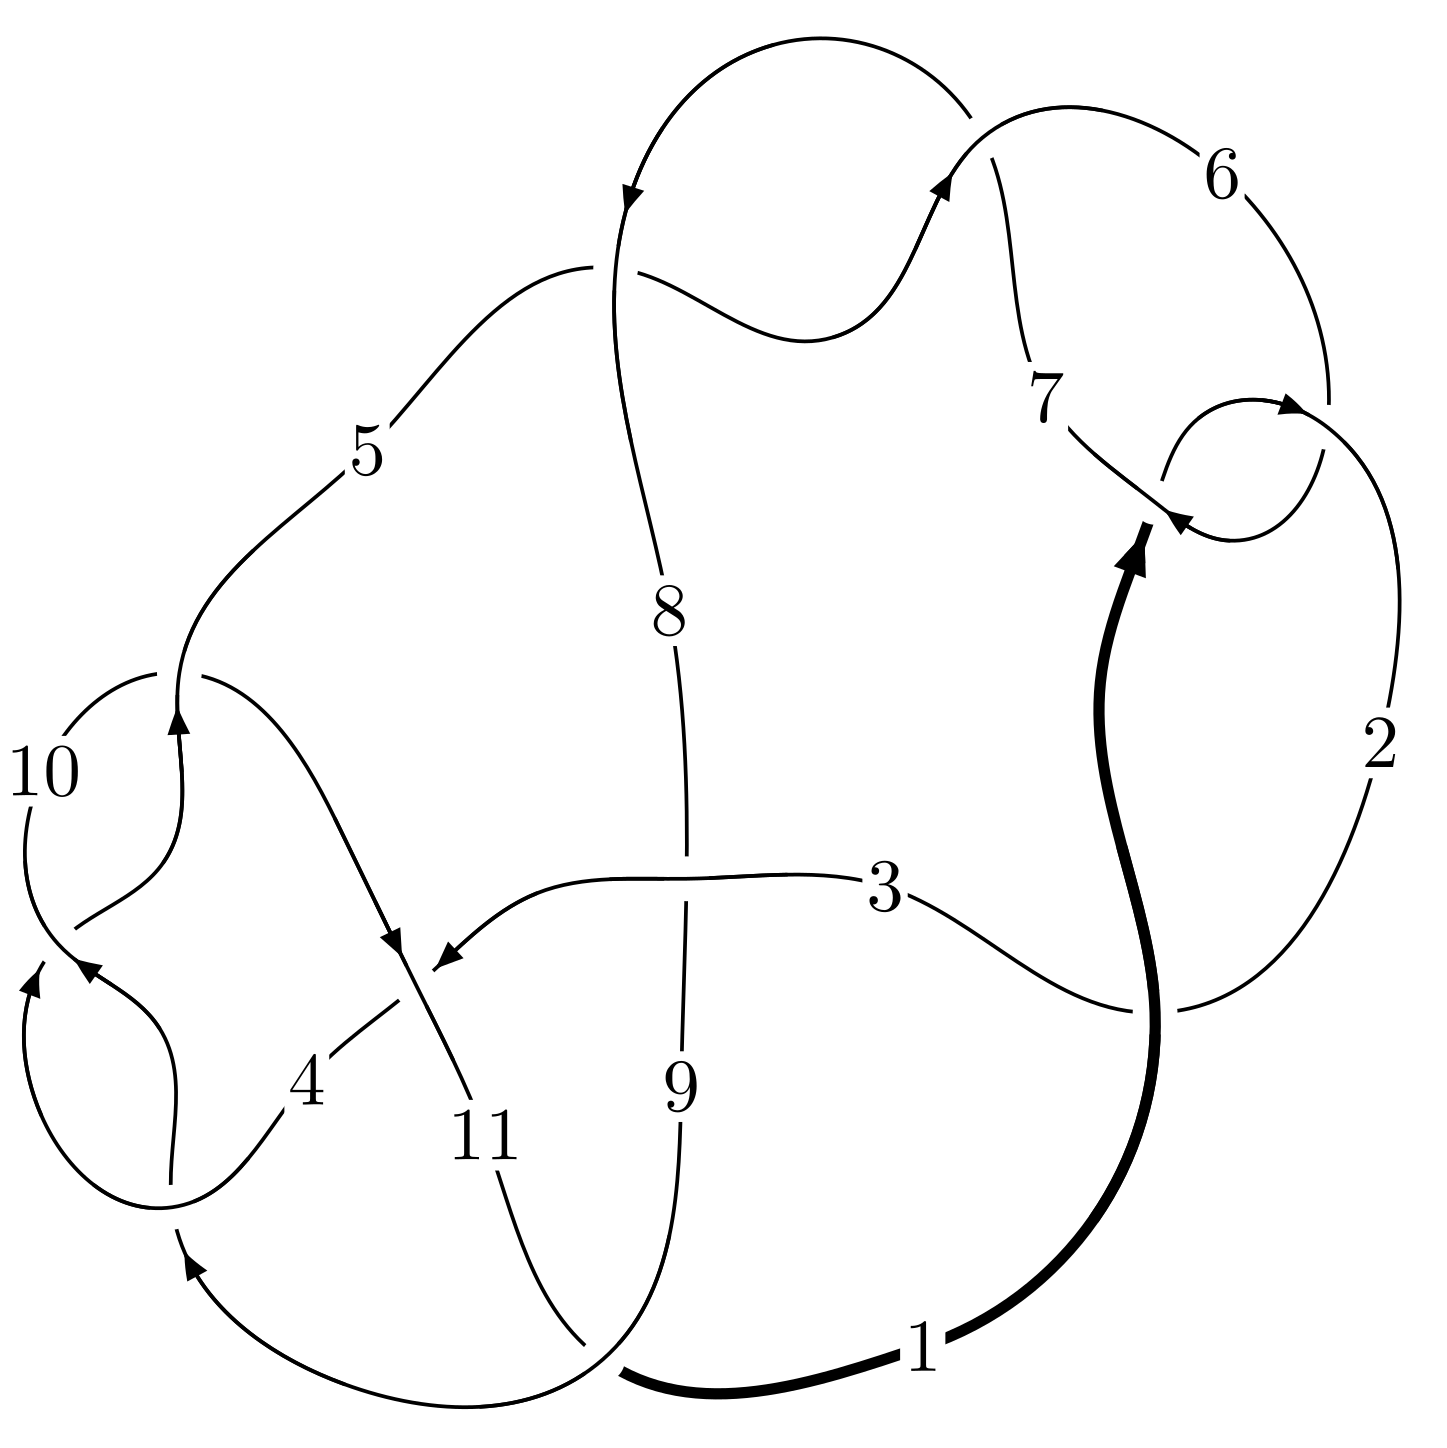
\includegraphics[width=112pt]{../../../GIT/diagram.site/Diagrams/png/454_11a_205.png}\\
\ \ \ A knot diagram\footnotemark}&
\allowdisplaybreaks
\textbf{Linearized knot diagam} \\
\cline{2-2}
 &
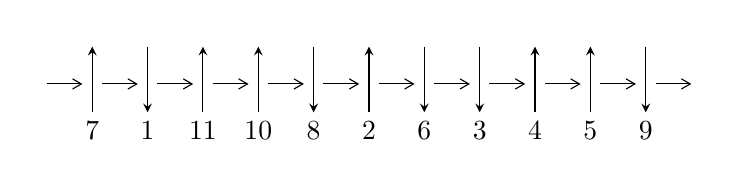
\begin{tikzpicture}[x=20pt, y=17pt]
	% nodes
	\node (C0) at (0, 0) {};
	\node (C1) at (1, 0) {};
	\node (C1U) at (1, +1) {};
	\node (C1D) at (1, -1) {7};

	\node (C2) at (2, 0) {};
	\node (C2U) at (2, +1) {};
	\node (C2D) at (2, -1) {1};

	\node (C3) at (3, 0) {};
	\node (C3U) at (3, +1) {};
	\node (C3D) at (3, -1) {11};

	\node (C4) at (4, 0) {};
	\node (C4U) at (4, +1) {};
	\node (C4D) at (4, -1) {10};

	\node (C5) at (5, 0) {};
	\node (C5U) at (5, +1) {};
	\node (C5D) at (5, -1) {8};

	\node (C6) at (6, 0) {};
	\node (C6U) at (6, +1) {};
	\node (C6D) at (6, -1) {2};

	\node (C7) at (7, 0) {};
	\node (C7U) at (7, +1) {};
	\node (C7D) at (7, -1) {6};

	\node (C8) at (8, 0) {};
	\node (C8U) at (8, +1) {};
	\node (C8D) at (8, -1) {3};

	\node (C9) at (9, 0) {};
	\node (C9U) at (9, +1) {};
	\node (C9D) at (9, -1) {4};

	\node (C10) at (10, 0) {};
	\node (C10U) at (10, +1) {};
	\node (C10D) at (10, -1) {5};

	\node (C11) at (11, 0) {};
	\node (C11U) at (11, +1) {};
	\node (C11D) at (11, -1) {9};
	\node (C12) at (12, 0) {};

	% arrows
	\draw[->,>={angle 60}]
	(C0) edge (C1) (C1) edge (C2) (C2) edge (C3) (C3) edge (C4) (C4) edge (C5) (C5) edge (C6) (C6) edge (C7) (C7) edge (C8) (C8) edge (C9) (C9) edge (C10) (C10) edge (C11) (C11) edge (C12) ;	\draw[->,>=stealth]
	(C1D) edge (C1U) (C2U) edge (C2D) (C3D) edge (C3U) (C4D) edge (C4U) (C5U) edge (C5D) (C6D) edge (C6U) (C7U) edge (C7D) (C8U) edge (C8D) (C9D) edge (C9U) (C10D) edge (C10U) (C11U) edge (C11D) ;
	\end{tikzpicture} \\
\hhline{~~} \\& 
\textbf{Solving Sequence} \\ \cline{2-2} 
 &
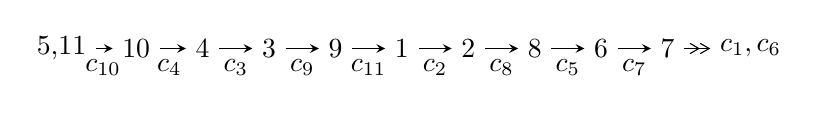
\begin{tikzpicture}[x=24pt, y=7pt]
	% node
	\node (A0) at (-1/8, 0) {5,11};
	\node (A1) at (1, 0) {10};
	\node (A2) at (2, 0) {4};
	\node (A3) at (3, 0) {3};
	\node (A4) at (4, 0) {9};
	\node (A5) at (5, 0) {1};
	\node (A6) at (6, 0) {2};
	\node (A7) at (7, 0) {8};
	\node (A8) at (8, 0) {6};
	\node (A9) at (9, 0) {7};
	\node (C1) at (1/2, -1) {$c_{10}$};
	\node (C2) at (3/2, -1) {$c_{4}$};
	\node (C3) at (5/2, -1) {$c_{3}$};
	\node (C4) at (7/2, -1) {$c_{9}$};
	\node (C5) at (9/2, -1) {$c_{11}$};
	\node (C6) at (11/2, -1) {$c_{2}$};
	\node (C7) at (13/2, -1) {$c_{8}$};
	\node (C8) at (15/2, -1) {$c_{5}$};
	\node (C9) at (17/2, -1) {$c_{7}$};
	\node (A10) at (41/4, 0) {$c_{1},c_{6}$};

	% edge
	\draw[->,>=stealth]	
	(A0) edge (A1) (A1) edge (A2) (A2) edge (A3) (A3) edge (A4) (A4) edge (A5) (A5) edge (A6) (A6) edge (A7) (A7) edge (A8) (A8) edge (A9) ;
	\draw[->>,>={angle 60}]	
	(A9) edge (A10);
\end{tikzpicture} \\ 

\end{tabular} \\

\footnotetext{
The image of knot diagram is generated by the software ``\textbf{Draw programme}" developed by Andrew Bartholomew(\url{http://www.layer8.co.uk/maths/draw/index.htm\#Running-draw}), where we modified some parts for our purpose(\url{https://github.com/CATsTAILs/LinksPainter}).
}\phantom \\ \newline 
\centering \textbf{Ideals for irreducible components\footnotemark of $X_{\text{par}}$} 
 
\begin{align*}
I^u_{1}&=\langle 
u^{45}- u^{44}+\cdots- u-1\rangle \\
\\
\end{align*}
\raggedright * 1 irreducible components of $\dim_{\mathbb{C}}=0$, with total 45 representations.\\
\footnotetext{All coefficients of polynomials are rational numbers. But the coefficients are sometimes approximated in decimal forms when there is not enough margin.}
\newpage
\renewcommand{\arraystretch}{1}
\centering \section*{I. $I^u_{1}= \langle u^{45}- u^{44}+\cdots- u-1 \rangle$}
\flushleft \textbf{(i) Arc colorings}\\
\begin{tabular}{m{7pt} m{180pt} m{7pt} m{180pt} }
\flushright $a_{5}=$&$\begin{pmatrix}0\\u\end{pmatrix}$ \\
\flushright $a_{11}=$&$\begin{pmatrix}1\\0\end{pmatrix}$ \\
\flushright $a_{10}=$&$\begin{pmatrix}1\\u^2\end{pmatrix}$ \\
\flushright $a_{4}=$&$\begin{pmatrix}- u\\- u^3+u\end{pmatrix}$ \\
\flushright $a_{3}=$&$\begin{pmatrix}u^3-2 u\\- u^3+u\end{pmatrix}$ \\
\flushright $a_{9}=$&$\begin{pmatrix}- u^2+1\\- u^4+2 u^2\end{pmatrix}$ \\
\flushright $a_{1}=$&$\begin{pmatrix}u^6-3 u^4+2 u^2+1\\u^8-4 u^6+4 u^4\end{pmatrix}$ \\
\flushright $a_{2}=$&$\begin{pmatrix}- u^{17}+8 u^{15}-25 u^{13}+36 u^{11}-19 u^9-4 u^7+2 u^5+4 u^3- u\\- u^{19}+9 u^{17}-32 u^{15}+55 u^{13}-43 u^{11}+9 u^9+4 u^5- u^3+u\end{pmatrix}$ \\
\flushright $a_{8}=$&$\begin{pmatrix}- u^{10}+5 u^8-8 u^6+3 u^4+u^2+1\\u^{10}-4 u^8+5 u^6-2 u^4+u^2\end{pmatrix}$ \\
\flushright $a_{6}=$&$\begin{pmatrix}- u^{21}+10 u^{19}+\cdots-2 u^3- u\\u^{21}-9 u^{19}+33 u^{17}-62 u^{15}+62 u^{13}-33 u^{11}+13 u^9-6 u^7+u^5- u^3+u\end{pmatrix}$ \\
\flushright $a_{7}=$&$\begin{pmatrix}- u^{32}+15 u^{30}+\cdots+2 u^2+1\\u^{32}-14 u^{30}+\cdots+2 u^6-2 u^4\end{pmatrix}$\\ \flushright $a_{7}=$&$\begin{pmatrix}- u^{32}+15 u^{30}+\cdots+2 u^2+1\\u^{32}-14 u^{30}+\cdots+2 u^6-2 u^4\end{pmatrix}$\\&\end{tabular}
\flushleft \textbf{(ii) Obstruction class $= -1$}\\~\\
\flushleft \textbf{(iii) Cusp Shapes $= -4 u^{42}+76 u^{40}+\cdots-4 u-2$}\\~\\
\newpage\renewcommand{\arraystretch}{1}
\flushleft \textbf{(iv) u-Polynomials at the component}\newline \\
\begin{tabular}{m{50pt}|m{274pt}}
Crossings & \hspace{64pt}u-Polynomials at each crossing \\
\hline $$\begin{aligned}c_{1},c_{6}\end{aligned}$$&$\begin{aligned}
&u^{45}+u^{44}+\cdots+u-1
\end{aligned}$\\
\hline $$\begin{aligned}c_{2},c_{5},c_{7}\end{aligned}$$&$\begin{aligned}
&u^{45}+11 u^{44}+\cdots- u-1
\end{aligned}$\\
\hline $$\begin{aligned}c_{3}\end{aligned}$$&$\begin{aligned}
&u^{45}+3 u^{44}+\cdots+7 u+3
\end{aligned}$\\
\hline $$\begin{aligned}c_{4},c_{9},c_{10}\end{aligned}$$&$\begin{aligned}
&u^{45}- u^{44}+\cdots- u-1
\end{aligned}$\\
\hline $$\begin{aligned}c_{8}\end{aligned}$$&$\begin{aligned}
&u^{45}+u^{44}+\cdots+44 u-40
\end{aligned}$\\
\hline $$\begin{aligned}c_{11}\end{aligned}$$&$\begin{aligned}
&u^{45}-9 u^{44}+\cdots+729 u-89
\end{aligned}$\\
\hline
\end{tabular}\\~\\
\newpage\renewcommand{\arraystretch}{1}
\flushleft \textbf{(v) Riley Polynomials at the component}\newline \\
\begin{tabular}{m{50pt}|m{274pt}}
Crossings & \hspace{64pt}Riley Polynomials at each crossing \\
\hline $$\begin{aligned}c_{1},c_{6}\end{aligned}$$&$\begin{aligned}
&y^{45}+11 y^{44}+\cdots- y-1
\end{aligned}$\\
\hline $$\begin{aligned}c_{2},c_{5},c_{7}\end{aligned}$$&$\begin{aligned}
&y^{45}+47 y^{44}+\cdots-9 y-1
\end{aligned}$\\
\hline $$\begin{aligned}c_{3}\end{aligned}$$&$\begin{aligned}
&y^{45}-5 y^{44}+\cdots+31 y-9
\end{aligned}$\\
\hline $$\begin{aligned}c_{4},c_{9},c_{10}\end{aligned}$$&$\begin{aligned}
&y^{45}-41 y^{44}+\cdots- y-1
\end{aligned}$\\
\hline $$\begin{aligned}c_{8}\end{aligned}$$&$\begin{aligned}
&y^{45}+7 y^{44}+\cdots-11024 y-1600
\end{aligned}$\\
\hline $$\begin{aligned}c_{11}\end{aligned}$$&$\begin{aligned}
&y^{45}+19 y^{44}+\cdots-92805 y-7921
\end{aligned}$\\
\hline
\end{tabular}\\~\\
\newpage\flushleft \textbf{(vi) Complex Volumes and Cusp Shapes}
$$\begin{array}{c|c|c}  
\text{Solutions to }I^u_{1}& \I (\text{vol} + \sqrt{-1}CS) & \text{Cusp shape}\\
 \hline 
\begin{aligned}
u &= -1.081740 + 0.103222 I\end{aligned}
 & -0.55475 - 2.53820 I & -1.85794 + 4.98062 I \\ \hline\begin{aligned}
u &= -1.081740 - 0.103222 I\end{aligned}
 & -0.55475 + 2.53820 I & -1.85794 - 4.98062 I \\ \hline\begin{aligned}
u &= \phantom{-}1.17086\phantom{ +0.000000I}\end{aligned}
 & \phantom{-}2.04246\phantom{ +0.000000I} & \phantom{-}5.49400\phantom{ +0.000000I} \\ \hline\begin{aligned}
u &= -1.177900 + 0.221582 I\end{aligned}
 & \phantom{-}5.59455 - 6.24371 I & \phantom{-}4.08567 + 6.12076 I \\ \hline\begin{aligned}
u &= -1.177900 - 0.221582 I\end{aligned}
 & \phantom{-}5.59455 + 6.24371 I & \phantom{-}4.08567 - 6.12076 I \\ \hline\begin{aligned}
u &= -0.327711 + 0.702255 I\end{aligned}
 & \phantom{-}5.55749 - 9.33109 I & \phantom{-}3.17264 + 7.99089 I \\ \hline\begin{aligned}
u &= -0.327711 - 0.702255 I\end{aligned}
 & \phantom{-}5.55749 + 9.33109 I & \phantom{-}3.17264 - 7.99089 I \\ \hline\begin{aligned}
u &= \phantom{-}0.336008 + 0.691887 I\end{aligned}
 & \phantom{-}5.95973 + 3.04960 I & \phantom{-}4.06449 - 3.14119 I \\ \hline\begin{aligned}
u &= \phantom{-}0.336008 - 0.691887 I\end{aligned}
 & \phantom{-}5.95973 - 3.04960 I & \phantom{-}4.06449 + 3.14119 I \\ \hline\begin{aligned}
u &= \phantom{-}1.213100 + 0.213850 I\end{aligned}
 & \phantom{-}5.84619 + 0.30511 I & \phantom{-}4.74215 + 0. I\phantom{ +0.000000I} \\ \hline\begin{aligned}
u &= \phantom{-}1.213100 - 0.213850 I\end{aligned}
 & \phantom{-}5.84619 - 0.30511 I & \phantom{-}4.74215 + 0. I\phantom{ +0.000000I} \\ \hline\begin{aligned}
u &= -0.591876 + 0.448289 I\end{aligned}
 & \phantom{-}6.60488 + 5.35917 I & \phantom{-}5.58298 - 2.28264 I \\ \hline\begin{aligned}
u &= -0.591876 - 0.448289 I\end{aligned}
 & \phantom{-}6.60488 - 5.35917 I & \phantom{-}5.58298 + 2.28264 I \\ \hline\begin{aligned}
u &= \phantom{-}0.568197 + 0.462450 I\end{aligned}
 & \phantom{-}6.90053 + 0.89679 I & \phantom{-}6.21998 - 2.86996 I \\ \hline\begin{aligned}
u &= \phantom{-}0.568197 - 0.462450 I\end{aligned}
 & \phantom{-}6.90053 - 0.89679 I & \phantom{-}6.21998 + 2.86996 I \\ \hline\begin{aligned}
u &= -0.269512 + 0.670457 I\end{aligned}
 & -1.92036 - 5.51147 I & -2.23282 + 8.80193 I \\ \hline\begin{aligned}
u &= -0.269512 - 0.670457 I\end{aligned}
 & -1.92036 + 5.51147 I & -2.23282 - 8.80193 I \\ \hline\begin{aligned}
u &= -0.019331 + 0.669875 I\end{aligned}
 & \phantom{-}2.10207 + 2.93926 I & -0.68998 - 2.61803 I \\ \hline\begin{aligned}
u &= -0.019331 - 0.669875 I\end{aligned}
 & \phantom{-}2.10207 - 2.93926 I & -0.68998 + 2.61803 I \\ \hline\begin{aligned}
u &= \phantom{-}0.283883 + 0.605501 I\end{aligned}
 & \phantom{-}0.18779 + 2.08707 I & \phantom{-}3.93114 - 4.06148 I \\ \hline\begin{aligned}
u &= \phantom{-}0.283883 - 0.605501 I\end{aligned}
 & \phantom{-}0.18779 - 2.08707 I & \phantom{-}3.93114 + 4.06148 I \\ \hline\begin{aligned}
u &= -0.174737 + 0.630370 I\end{aligned}
 & -3.06951 - 0.40423 I & -6.40296 + 0.79013 I \\ \hline\begin{aligned}
u &= -0.174737 - 0.630370 I\end{aligned}
 & -3.06951 + 0.40423 I & -6.40296 - 0.79013 I \\ \hline\begin{aligned}
u &= \phantom{-}1.370030 + 0.236669 I\end{aligned}
 & \phantom{-}1.84057 + 3.53925 I & \phantom{-0.000000 } 0 \\ \hline\begin{aligned}
u &= \phantom{-}1.370030 - 0.236669 I\end{aligned}
 & \phantom{-}1.84057 - 3.53925 I & \phantom{-0.000000 } 0 \\ \hline\begin{aligned}
u &= \phantom{-}1.389940 + 0.138970 I\end{aligned}
 & \phantom{-}5.13702 - 0.60420 I & \phantom{-0.000000 } 0 \\ \hline\begin{aligned}
u &= \phantom{-}1.389940 - 0.138970 I\end{aligned}
 & \phantom{-}5.13702 + 0.60420 I & \phantom{-0.000000 } 0 \\ \hline\begin{aligned}
u &= -0.535574 + 0.250743 I\end{aligned}
 & -0.56423 + 2.11330 I & \phantom{-}1.09230 - 3.69401 I \\ \hline\begin{aligned}
u &= -0.535574 - 0.250743 I\end{aligned}
 & -0.56423 - 2.11330 I & \phantom{-}1.09230 + 3.69401 I \\ \hline\begin{aligned}
u &= -1.40867 + 0.18655 I\end{aligned}
 & \phantom{-}6.35213 - 3.35003 I & \phantom{-0.000000 } 0\\
 \hline 
 \end{array}$$\newpage$$\begin{array}{c|c|c}  
\text{Solutions to }I^u_{1}& \I (\text{vol} + \sqrt{-1}CS) & \text{Cusp shape}\\
 \hline 
\begin{aligned}
u &= -1.40867 - 0.18655 I\end{aligned}
 & \phantom{-}6.35213 + 3.35003 I & \phantom{-0.000000 } 0 \\ \hline\begin{aligned}
u &= -1.41039 + 0.23841 I\end{aligned}
 & \phantom{-}5.60817 - 5.19685 I & \phantom{-0.000000 } 0 \\ \hline\begin{aligned}
u &= -1.41039 - 0.23841 I\end{aligned}
 & \phantom{-}5.60817 + 5.19685 I & \phantom{-0.000000 } 0 \\ \hline\begin{aligned}
u &= \phantom{-}1.40670 + 0.26177 I\end{aligned}
 & \phantom{-}3.43096 + 8.91009 I & \phantom{-0.000000 } 0 \\ \hline\begin{aligned}
u &= \phantom{-}1.40670 - 0.26177 I\end{aligned}
 & \phantom{-}3.43096 - 8.91009 I & \phantom{-0.000000 } 0 \\ \hline\begin{aligned}
u &= \phantom{-}0.346105 + 0.427336 I\end{aligned}
 & \phantom{-}0.805234 + 0.974268 I & \phantom{-}6.02798 - 5.00492 I \\ \hline\begin{aligned}
u &= \phantom{-}0.346105 - 0.427336 I\end{aligned}
 & \phantom{-}0.805234 - 0.974268 I & \phantom{-}6.02798 + 5.00492 I \\ \hline\begin{aligned}
u &= \phantom{-}1.43383 + 0.27147 I\end{aligned}
 & \phantom{-}11.2002 + 12.8798 I & \phantom{-0.000000 } 0 \\ \hline\begin{aligned}
u &= \phantom{-}1.43383 - 0.27147 I\end{aligned}
 & \phantom{-}11.2002 - 12.8798 I & \phantom{-0.000000 } 0 \\ \hline\begin{aligned}
u &= -1.43584 + 0.26614 I\end{aligned}
 & \phantom{-}11.63810 - 6.54354 I & \phantom{-0.000000 } 0 \\ \hline\begin{aligned}
u &= -1.43584 - 0.26614 I\end{aligned}
 & \phantom{-}11.63810 + 6.54354 I & \phantom{-0.000000 } 0 \\ \hline\begin{aligned}
u &= \phantom{-}1.45671 + 0.13963 I\end{aligned}
 & \phantom{-}13.09220 - 3.34284 I & \phantom{-0.000000 } 0 \\ \hline\begin{aligned}
u &= \phantom{-}1.45671 - 0.13963 I\end{aligned}
 & \phantom{-}13.09220 + 3.34284 I & \phantom{-0.000000 } 0 \\ \hline\begin{aligned}
u &= -1.45665 + 0.14856 I\end{aligned}
 & \phantom{-}13.32800 - 3.02786 I & \phantom{-0.000000 } 0 \\ \hline\begin{aligned}
u &= -1.45665 - 0.14856 I\end{aligned}
 & \phantom{-}13.32800 + 3.02786 I & \phantom{-0.000000 } 0\\
 \hline 
 \end{array}$$\newpage
\newpage\renewcommand{\arraystretch}{1}
\centering \section*{ II. u-Polynomials}
\begin{tabular}{m{50pt}|m{274pt}}
Crossings & \hspace{64pt}u-Polynomials at each crossing \\
\hline $$\begin{aligned}c_{1},c_{6}\end{aligned}$$&$\begin{aligned}
&u^{45}+u^{44}+\cdots+u-1
\end{aligned}$\\
\hline $$\begin{aligned}c_{2},c_{5},c_{7}\end{aligned}$$&$\begin{aligned}
&u^{45}+11 u^{44}+\cdots- u-1
\end{aligned}$\\
\hline $$\begin{aligned}c_{3}\end{aligned}$$&$\begin{aligned}
&u^{45}+3 u^{44}+\cdots+7 u+3
\end{aligned}$\\
\hline $$\begin{aligned}c_{4},c_{9},c_{10}\end{aligned}$$&$\begin{aligned}
&u^{45}- u^{44}+\cdots- u-1
\end{aligned}$\\
\hline $$\begin{aligned}c_{8}\end{aligned}$$&$\begin{aligned}
&u^{45}+u^{44}+\cdots+44 u-40
\end{aligned}$\\
\hline $$\begin{aligned}c_{11}\end{aligned}$$&$\begin{aligned}
&u^{45}-9 u^{44}+\cdots+729 u-89
\end{aligned}$\\
\hline
\end{tabular}\newpage\renewcommand{\arraystretch}{1}
\centering \section*{ III. Riley Polynomials}
\begin{tabular}{m{50pt}|m{274pt}}
Crossings & \hspace{64pt}Riley Polynomials at each crossing \\
\hline $$\begin{aligned}c_{1},c_{6}\end{aligned}$$&$\begin{aligned}
&y^{45}+11 y^{44}+\cdots- y-1
\end{aligned}$\\
\hline $$\begin{aligned}c_{2},c_{5},c_{7}\end{aligned}$$&$\begin{aligned}
&y^{45}+47 y^{44}+\cdots-9 y-1
\end{aligned}$\\
\hline $$\begin{aligned}c_{3}\end{aligned}$$&$\begin{aligned}
&y^{45}-5 y^{44}+\cdots+31 y-9
\end{aligned}$\\
\hline $$\begin{aligned}c_{4},c_{9},c_{10}\end{aligned}$$&$\begin{aligned}
&y^{45}-41 y^{44}+\cdots- y-1
\end{aligned}$\\
\hline $$\begin{aligned}c_{8}\end{aligned}$$&$\begin{aligned}
&y^{45}+7 y^{44}+\cdots-11024 y-1600
\end{aligned}$\\
\hline $$\begin{aligned}c_{11}\end{aligned}$$&$\begin{aligned}
&y^{45}+19 y^{44}+\cdots-92805 y-7921
\end{aligned}$\\
\hline
\end{tabular}
\vskip 2pc
\end{document}